\chapter{Unidad VI.}
\section{
	Seguridad Informática
}
La seguridad informática,\textbf{ es el conjunto de prácticas, procesos, técnicas y tecnologías diseñadas para proteger los sistemas informáticos, redes, programas, datos y dispositivos contra amenazas, ataques y accesos no autorizados.}
\subsection{Objetivos de la seguridad informática}
 El objetivo principal de la seguridad informática es garantizar la confidencialidad, integridad y disponibilidad de la información almacenada y procesada en entornos digitales.
 \subsubsection{Confidencialidad}
 Los  datos solo pueden ser legibles y modificados por personas autorizadas, tanto en el acceso a datos almacenados como también durante la transferencia de ellos.

\subsubsection{Integridad}
Los datos están completos, sin modificar y todos los cambios son reproducibles (se conoce el autor y el momento del cambio). Solo quienes tengan la debida autorización podrán eliminar, descargar o modificar datos.
\subsubsection{Disponibilidad}
El acceso a los datos debe ser garantizado en el momento necesario. Hay que evitar fallos del sistema y proveer el acceso adecuado.
\section{Antivirus}
 Un antivirus\textbf{ es un programa diseñado para detectar, prevenir y eliminar software malicioso (malware) de los sistemas informáticos.} El término ``antivirus'' a menudo se utiliza de manera más general para referirse a programas de seguridad que abordan no solo virus tradicionales, sino también otras formas de malware, como gusanos, troyanos, spyware, ransomware y más.
\subsection{Modos de detección que emplean los antivirus}
 \begin{tcolorbox}[title= Modos de detección que emplean los antivirus]
 	\begin{itemize}
 		
 		
 		\item \textbf{Escaneo:}
 		Un antivirus analiza archivos y programas en busca de patrones o comportamientos sospechosos que puedan indicar la presencia de malware. Utiliza bases de datos de firmas y técnicas de análisis heurístico para identificar amenazas conocidas y nuevas.
 		\item \textbf{Detección de Firmas (Signature-Based):}
 		 Este método se basa en el uso de firmas o patrones específicos conocidos de malware. Las firmas son características únicas de fragmentos de código de malware identificados previamente
 		\item \textbf{Detección de Comportamiento:}
 		Al observar el comportamiento de programas y procesos en tiempo real, los antivirus pueden detectar actividades maliciosas. Por ejemplo, si un programa intenta modificar archivos de sistema sin autorización, el antivirus podría identificarlo como una amenaza.
 		 
 		
 	\end{itemize}
 \end{tcolorbox}
 \section{Firewall}
 Un firewall es un componente de seguridad informática que actúa como una barrera entre una red privada y redes externas, como Internet. Su función principal es controlar y monitorear el tráfico de red, permitiendo o bloqueando la comunicación basándose en un conjunto de reglas predefinidas.
 \subsection{Tipos de firewall}
 \subsubsection{Firewalls de hardware}
  Son dispositivos físicos independientes que se colocan entre la red interna y la externa. Pueden ser dispositivos dedicados o integrados en enrutadores y otros dispositivos de red.
 
 \begin{figure}[H]
 	\centering
 	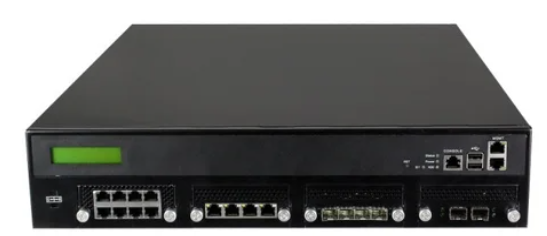
\includegraphics[width=0.4\linewidth]{Imagenes/firewall.png}
 	\caption{ Los firewalls pueden ser dispositivos físicos independientes, colocados entre la red interna y externa. }
 	\label{fig:enter-label}
 \end{figure}
 \subsubsection{Firewalls de software}
  Son programas o aplicaciones que se ejecutan en sistemas operativos y proporcionan funciones de firewall. Pueden ser instalados en servidores, computadoras personales o incluso dispositivos móviles.
  
  \subsection{Funciones principales de un firewall}
  \begin{tcolorbox}[title= Funcionamiento básico de un firewall]
  	\begin{itemize}
  		
  		
  		\item \textbf{Filtrado de Paquetes (Packet Filtering):}
  		Examina la información de encabezado de los paquetes de datos y decide si permitir o bloquear el paso según reglas específicas. Las reglas pueden basarse en direcciones de IP, puertos, protocolos, y otros atributos del paquete.
  		\item \textbf{Inspección de Estado (Stateful Inspection):}
  		Realiza un seguimiento del estado de las conexiones y toma decisiones basadas en el contexto, permitiendo o bloqueando el tráfico en función del estado de la conexión. Si un paquete pertenece a una conexión establecida y permitida, es más probable que se le permita.
  		\item \textbf{Logging y Auditoría:}
  		Los firewalls registran eventos y actividades, como conexiones exitosas o bloqueadas. Estos registros son esenciales para la auditoría de seguridad, la resolución de problemas y la identificación de patrones de tráfico anómalos.
  		
  		
  	\end{itemize}
  \end{tcolorbox}